%%
%% 研究報告用スイッチ(情報処理学会用ファイルをEC2014用に変更)
%% [techrep]
%%
%% 欧文表記無しのスイッチ(etitle,jkeyword,eabstract,ekeywordは任意)
%% [noauthor]
%%
\documentclass[report,10pt,uplatex,titlepage]{jsarticle}
\usepackage[dvips]{graphicx}
\usepackage[hyphens]{url}

\listfiles

%% 読み込みファイル 一覧表示
\begin{document}


\title{卒業論文中間報告\vspace{5mm}\\笑い声提示により自然な笑顔を\\撮影するカメラの基礎検討}
\author{03-130452\\伏見 遼平}
\maketitle

\thispagestyle{empty} % ページ数を表示しない

\tableofcontents % 目次

\thispagestyle{empty} % ページ数を表示しない


\pagebreak

\section{はじめに}

%% ページ数のカウンタを上書き.最初のsectionの後じゃないとダメ
\setcounter{page}{1}

記念撮影やポートレートなどの人物写真において,自然な表情を撮影するのは難しい.「ハイチーズ」「笑って!」など,カメラマンが被撮影者に言語的な働きかけを行うことも多いが,これにより笑顔を作るように誘導したとしても,作り笑いになることが多い.

% (「自然な笑顔」ぼくたちが自然な笑顔をどういうものだと思っているかを示す.ハイチーズみたいな笑い方,自然な表情であるかは微妙.イラストでこれやりたいが分かる2枚)
% カメラは被写体のありのままの姿を記録するためにデザインされている.ストロボなどを除けば、基本的にはカメラや付属する機器は被写体に対して働きかけを行うものは少ない.しかし、ポートレートなどの人物写真については、被写体となる人間とのコミュニケーションも重要である.カメラマンからは「ハイチーズ」「笑って」などの声掛けがなされるが,言語でコミュニケーションを取ったり,笑顔を作るように誘導したとしても,随意的な笑顔しか撮影することができない.

\begin{figure}[b!]

\begin{minipage}{0.14\columnwidth}\vspace{10 mm}\hspace{20 mm}
\end{minipage}
\begin{minipage}{0.35\columnwidth}
\begin{center}
\includegraphics[width=40mm, bb=0 0 768 1024]{images/smile-non-duchenne.jpg}
\end{center}
\end{minipage}
\begin{minipage}{0.35\columnwidth}
\begin{center}
\includegraphics[width=40mm, bb=0 0 768 1024]{images/smile-duchenne.jpg}
\end{center}
\end{minipage}
\begin{minipage}{0.14\columnwidth}
\end{minipage}

\label{hirashimasmile}
\begin{center}
\caption{左: 作り笑いの笑顔 右: 本研究の目指す自然な笑顔}

\end{center}
\end{figure}

私は現在,カメラそのものが被撮影者の情動に直接働きかけ,笑顔を誘発するようなカメラシステムを研究している.笑顔を誘発するために,つられ笑いや思い出し笑いなどの非随意的なメカニズムを使えば,自然な笑顔が撮影できる可能性があることに着目した.図\ref{hirashimasmile}に本研究の目指すイメージを参考画像として示した.

本研究では,他者の笑いが笑いを誘発する効果を利用して,シャッターを切る前に笑い声を再生することで自然な笑顔を撮影するカメラシステム"爆笑カメラ"を提案する.その実証のために,システムをスマートフォン上で動作するアプリケーションとして実装し,実際に効果を検討した.まず,予備実験として事前に収集した笑顔を誘発しやすい笑い声音声素材の中から最も笑顔の誘発に効果的である素材を選定した.次に実験室の統制された環境で,2種類の笑い声音声と通常のシャッター音で撮影された笑顔にどのような違いがあるかに加えて,効果が現れるタイミングと効果の男女差を検討した.

%2
\section{関連研究}

ここでは,人の笑顔のメカニズムに関する知見を整理し,私が目指す笑顔の種類について言及する.次に写真撮影のシーンにおいて,被撮影者に働きかける事例を撮影者から被撮影者に働きかける事例とカメラシステムから被撮影者に働きかける事例に分類する.さらにそれぞれの分類の中で,働きかけの方法を言語的なものと非言語的なものに分け,それぞれの特長を整理する.

\subsection{人の笑顔のメカニズムに関する知見}

Duchenneは,人の笑顔には2つの異なるタイプがあると指摘した.大頬骨筋と眼輪筋両方の動きが観察されるDuchenne Smileと,大頬骨筋のみの動きしか見られないnon-Duchenne Smileである\cite{de1990mechanism}.このうち眼輪筋は不随意であり,Duchenne Smile こそが真の笑い,「魂の喜ばしい衝動」であり,non-Duchenne Smileは愛想笑いの表出であるとしている.Surakkaらは前者と後者の筋肉の動きの差をEMGを用いて調査し,それぞれに対応する筋肉群をまとめた \cite{surakka1998facial}.これら2種の笑顔の表出は,単に使われる筋肉が異なるというだけはなく,表情筋の情動性の制御を担う脳の経路は,同じ筋肉の随意的な制御を担う部位とは異なることもわかっている\cite{tanaka201007}.Ekmanは自然な笑いと作り笑いの違いについて,作り笑いは自然な笑いに比べ,眼輪筋の筋肉の動きを伴わないのに加えて,左右非対称であることを指摘している\cite{ekman2009telling}.

私の提案するシステムが目指すのはDuchenne Smile,すなわち意識して表出できるものではない不随意の眼輪筋の収縮を伴う笑顔であり,これを論文中では「自然な笑い」と呼ぶ.

\subsection{撮影者から被撮影者への働きかけ}

記念撮影のシーンにおいてカメラマンによる被撮影者への語りかけや掛け声が多くみられ,これには位置やポーズ,表情についての指示だけではなく,被撮影者をリラックスさせようという意図の語りかけも多く見られる.このような言語的アプローチは被撮影者に表情の指示を細かく伝えることができる点で有効だが,これは随意的な笑顔になりがちである.トークなどを通じて非随意的な笑いを意識して引き出すことのできるカメラマンも存在するが,個々のスキルに依存する.

「チーズ」「ミッキー」などの語末に /i/ 音がある単語を発音させ,口角を上げさせる撮影の手法もある.これは笑顔の表情筋の使い方に
笑顔を撮影するのに有効な方法であるが,これも随意的な笑顔だと考えられる.

\subsection{カメラシステムから被撮影者への働きかけ}



市販カメラのうちキヤノン社の一部機種(IXY DIGITAL 930IS, Powershot G11など)では,ユーザが付属ソフトでシャッター音を設定できるものがある\cite{PowershotG1X}.ガラケーと呼ばれる日本製フィーチャーフォンでもシャッター音を設定できる機能がある.これらのシステムは実際のシャッターが下りるのと同時に音声を鳴らすものであり,シャッターを切る前に音声再生によって撮りたい表情を引き出すという本研究のアプローチとは異なるものである.

プリクラ撮影機では,具体的な表情やポーズ等の指示について事前収録された音声が再生される.この指示は意識的な笑顔や"変顔"を表出させる言語的な働きかけである.プリクラ撮影機では他にも音楽や照明など撮影シーンを盛り上げる様々な試みがなされている.単体のカメラの実装を目指すにあたり,参考にできるものがあるだろう.

D2Cのリリースしたスマートフォン向けアプリ「笑顔が撮れる こどもカメラ」は,幼児の自然な笑顔を写真におさめるためのアプリケーションである\cite{kodomocamera}.スマートフォンの画面にキャラクターを表示させ,これを動かすことで幼児の興味を引き,シャッターを切る.これは撮影しにくい子供の笑顔を気を引くことにより撮影するためのものであり,本研究に近い事例である.

%\begin{figure}[h!]
%  \centering  
%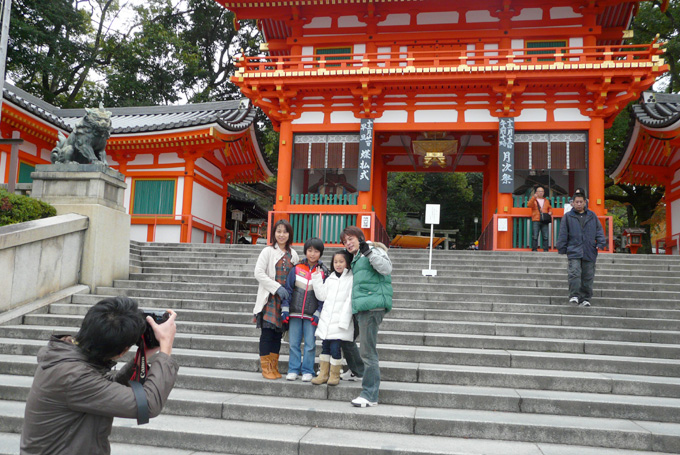
\includegraphics[width=55mm, bb=0 0 680 455]{images/murataphoto-main.jpg}
%\caption{プロカメラマンの写真撮影の例}
%  \label{pro-cameraman}
%\end{figure}

%% ※ 表

\subsection{笑い声呈示による笑い誘発}

私は,カメラシステムからの働きかけの中で非随意な笑顔を誘発するために,他者の笑い声を利用する事を検討する.笑い声の伝染現象は古くから研究されている.Provineは,この伝染現象は学習ではなく無意識的で生得的な行動であることを指摘している\cite{provine1996laughter}.またProvineは,心理学の講義を履修した128名の学生に対し,18秒間の笑い声を聞かせ,42秒間の間を空けることを10回繰り返し,それぞれの試行について笑顔になったか否かおよび笑ったか否かを報告させた\cite{provine1992contagious}.繰り返しにより笑顔・笑いを誘発できた割合は大きく下がり,繰り返しの後半では不快感を感じたという報告も多かった. Platowらは,社会的に近い集団による笑い声の方が,そうでない集団の笑い声よりも笑いの伝染を引き起こしやすいことを指摘している\cite{platow41n}.

陰山らは,快感情を伴う自然な笑いと伴わない作り笑いによる情動の伝染について研究したが,自然な笑いか作り笑いかという表出の種別よりも,被験者が笑いを自然だと感じたかが情動の伝染において重要であることを報告している\cite{蔭山2005}.誘発に用いる笑い声自体は必ずしも自然な笑いによるものである必要はないことが示唆される.

次に笑い誘発を実世界のデバイスに応用した例について取り上げる.「笑い袋」は,1969年ごろ流行したおもちゃで,ボタンを押すとシュールな笑い声がとめどなく流れるというものである.現在はぬいぐるみに内蔵された「わらいぶくろベイビーズ」という商品が販売されている\cite{waraibukurobabies}.「くすぐりエルモ (Tickle me Elmo)」\cite{ticklemeelmo}は,子供に人気のキャラクター「エルモ」のぬいぐるみであるが,腹部を触るとエルモが笑い転げる.嶋本らは,プレゼンテーション時に聴衆のPCから笑い声を再生し,笑いや拍手を誘発するシステムを提案している\cite{shimamoto2013}.また笑い声を音声や映像コンテンツへ応用した事例は多く存在し,一般的にlaugh track(ラフトラック)と呼ばれる.ジョーク集にラフトラックを付加することで,人の笑いが増幅されたという研究成果が報告されている\cite{chapman1973funniness}.福嶋らはこれらの研究を元に「笑い増幅器」を提案し,実装した\cite{fukushima2010}.私はこの誘発メカニズムをカメラ撮影のインターフェイスに応用したシステムを提案する.

\section{システム}

本システムでは,笑い声を被撮影者に呈示しながら写真を撮影する必要がある.一眼レフなどのデジタルカメラのシャッターと同期して音声を再生する装置を検討したが,同期のための機構が必要となってしまう.また,複雑な装置のセットアップが必要なシステムでは,結局のところ「誰でも自然な笑顔が撮影できる」という目的に適わない.同期を簡便に実現でき,音声再生から撮影までの遅延を自由に制御でき,さらに簡単にセットアップできるという利点を持つスマートフォン向けのアプリケーションとして実装した.
図\ref{ss1}, \ref{ss2} にスクリーンショットを示す.

\begin{figure}[h] 
\begin{minipage}{0.49\columnwidth}
\begin{center}
\includegraphics[width=60mm, bb=0 0 631 1024]{images/ss/ss1-resized.jpg}
\caption{サウンド音量確認画面}
\label{ss1}
\end{center}
\end{minipage}
\begin{minipage}{0.49\columnwidth}
\begin{center}
\includegraphics[width=60mm, bb=0 0 631 1024]{images/ss/ss2-resized.jpg}
\caption{撮影画面}
\label{ss2}
\end{center}
\end{minipage}
\end{figure}


本システムはスマートフォン,スピーカによって構成されている.事前にインストールした音声を選択し,ボタンを押した時刻から音声を再生しながら録画を始め,タイマーで音声を再生し,録画をストップするアプリケーションをObjective-Cで記述し,iOSのスマートフォンにインストールした.アプリケーションは通常の写真撮影モードと,動画を撮影するモードを持つ.

一般向けの写真撮影アプリケーションとして配布しデータを収集することを見込み,著者以外でも実験ができるように教示をアプリケーションの画面の中に埋め込んだ.


\section{予備実験}

本実験で使用する音声の種類を選定するために予備実験を行った.下記に示す5種類の笑い声を用意し,3人の被験者 (男性2名,女性1名) に聴かせて,表情を観察し感想を聞いた.笑顔を誘発する効果の大きかった (1)幼児の笑い声 (3)青年の笑い声を本実験に用いることにした.音声データはロイヤリティフリーの音声素材を提供するWebサイトaudioblocks\cite{AudioBlocks}から取得した.

\begin{enumerate}
 \item 幼児の笑い声 (12秒)
 \item 少年の笑い声 (10秒)
 \item 青年の笑い声 (15秒)
 \item 青年の3名の笑い声 (11秒)
 \item 多人数の笑い声 (ラフトラック) (12秒)
\end{enumerate}

\section{実験}

\subsection{目的}

システムが有効に笑顔を誘発できているかを確かめるため,実験室で本システムを使って撮影した画像群について,「Rekognition API」を用いて笑顔尺度を測定し,システムの効果を検証した.もっとも効果が現れるタイミング,音声の種類と男女要因の交互作用を検討した.

\subsection{実験条件および実験設備環境}


21-36歳の被験者19名に対して実験を行った.実験は静かな実験室で,実験者と二人の状況で行われた.実験条件として,音声を予備実験で選定した「(3)青年の笑い声」「(1)幼児の笑い声」「一眼レフカメラのオートフォーカス合焦音+シャッター音(対照条件)」に設定した3条件(表\ref{cond5})で実験を行った.カメラデバイスをスタンドに設置し,実験者はスタンドの右斜め後ろで被験者に教示を与えたのち,デバイスを操作した.実験用にセットアップしたシステムの外観及び実験の様子を図\ref{system}, \ref{yousu}に示した.

\begin{figure}[h!]
\begin{minipage}{0.49\columnwidth}
\begin{center}
\includegraphics[width=70mm, bb=0 0 768 1024]{images/system-resized.jpg}
\end{center}
\caption{システムの外観}
  \label{system}
\end{minipage}
\begin{minipage}{0.49\columnwidth}
\begin{center}
\includegraphics[width=70mm, bb=0 0 768 1024]{images/DSC05173-resized.jpg}
\end{center}
\caption{実験の様子}
  \label{yousu}
\end{minipage}
\end{figure}

\break

なお被験者の属性は東京大学・東京外国語大学の学生および東京大学の大学職員であった (男性8名, 女性11名, 平均23.1歳) .
\begin{table}[htb]
  \begin{center}
    \caption{実験条件}
    \label{cond5}
    \begin{tabular}{|l|c|c|} \hline
      条件 & 音声の内容 & 継続時間 \\ \hline  \hline
      条件1 & 青年の笑い声 & 9秒\\ \hline 
      条件2 & 幼児の笑い声 & 9秒 \\ \hline
      条件3 & デジタルカメラの合焦音+シャッター音 (対照) & 2秒 \\ \hline
    \end{tabular}
  \end{center}
\end{table}




\subsection{手続き}
\label{手続き}

被験者には,この実験は写真を撮る際のシャッター音の表情への影響を調べる実験であることが伝えられ,「いつも写真に撮られるときの笑顔で映ってください」という教示が与えられた.すなわち3条件とも,音声の呈示がある前は随意的な「作り笑顔」を作った状態から,音声が呈示された.

さらに注意としてシャッター音には長いものも短いものもあること,撮影中はなるべくカメラレンズを見つめるようにすることを伝えたのち,3条件で撮影を行った.順序効果を相殺するため,実験条件の順序はラテン方格法により割り当てられた.3条件すべての撮影後,それぞれの体験についてどういう感想を持ったかを聞いた.


\subsection{評価方法}

撮影された8秒間の動画から,$15 [fps]$で静止画像を切り出し,条件間の表情の差異,および表情の時間変化について分析を行った.

切り出しにはffmpegを用い,以下のコマンドオプションを用いた.

\begin{verbatim}
$ ffmpeg -i %s -vf "transpose=1" -s 1080x1920 -qscale:v 0 -r 15 ../captures/%s/cap_%%02d.jpg
\end{verbatim}

その後まず,Rekognition APIを用いて,各画像の笑顔尺度の測定を行った.Rekognition APIはOrbeus社による表情認識APIで,画像を送信すると表情を解析し,0〜1の値で笑顔尺度を返す.この値を顔全体の笑顔の度合いとみなし,値の時間変化と条件間の差異を分析した.

ただし,目を閉じている場合,笑顔尺度は目を閉じていない前後のフレームよりも大きく値が低下する.このことから,目を閉じていると判定されたフレームとその前後2フレームについては,3フレーム前の笑顔尺度の値と3フレーム後の笑顔尺度の値の平均値を採用した.

\subsection{結果と考察}

笑顔尺度の時間変化を条件ごとに平均した値をプロットしたものを図\ref{graph-smooth}に示す.表\ref{cond5}の通り,プロットした時間区間の間は条件1,2ではずっと音声が流れていたが,条件3では無音の区間も含む.

\begin{figure}[h!]
  \centering  
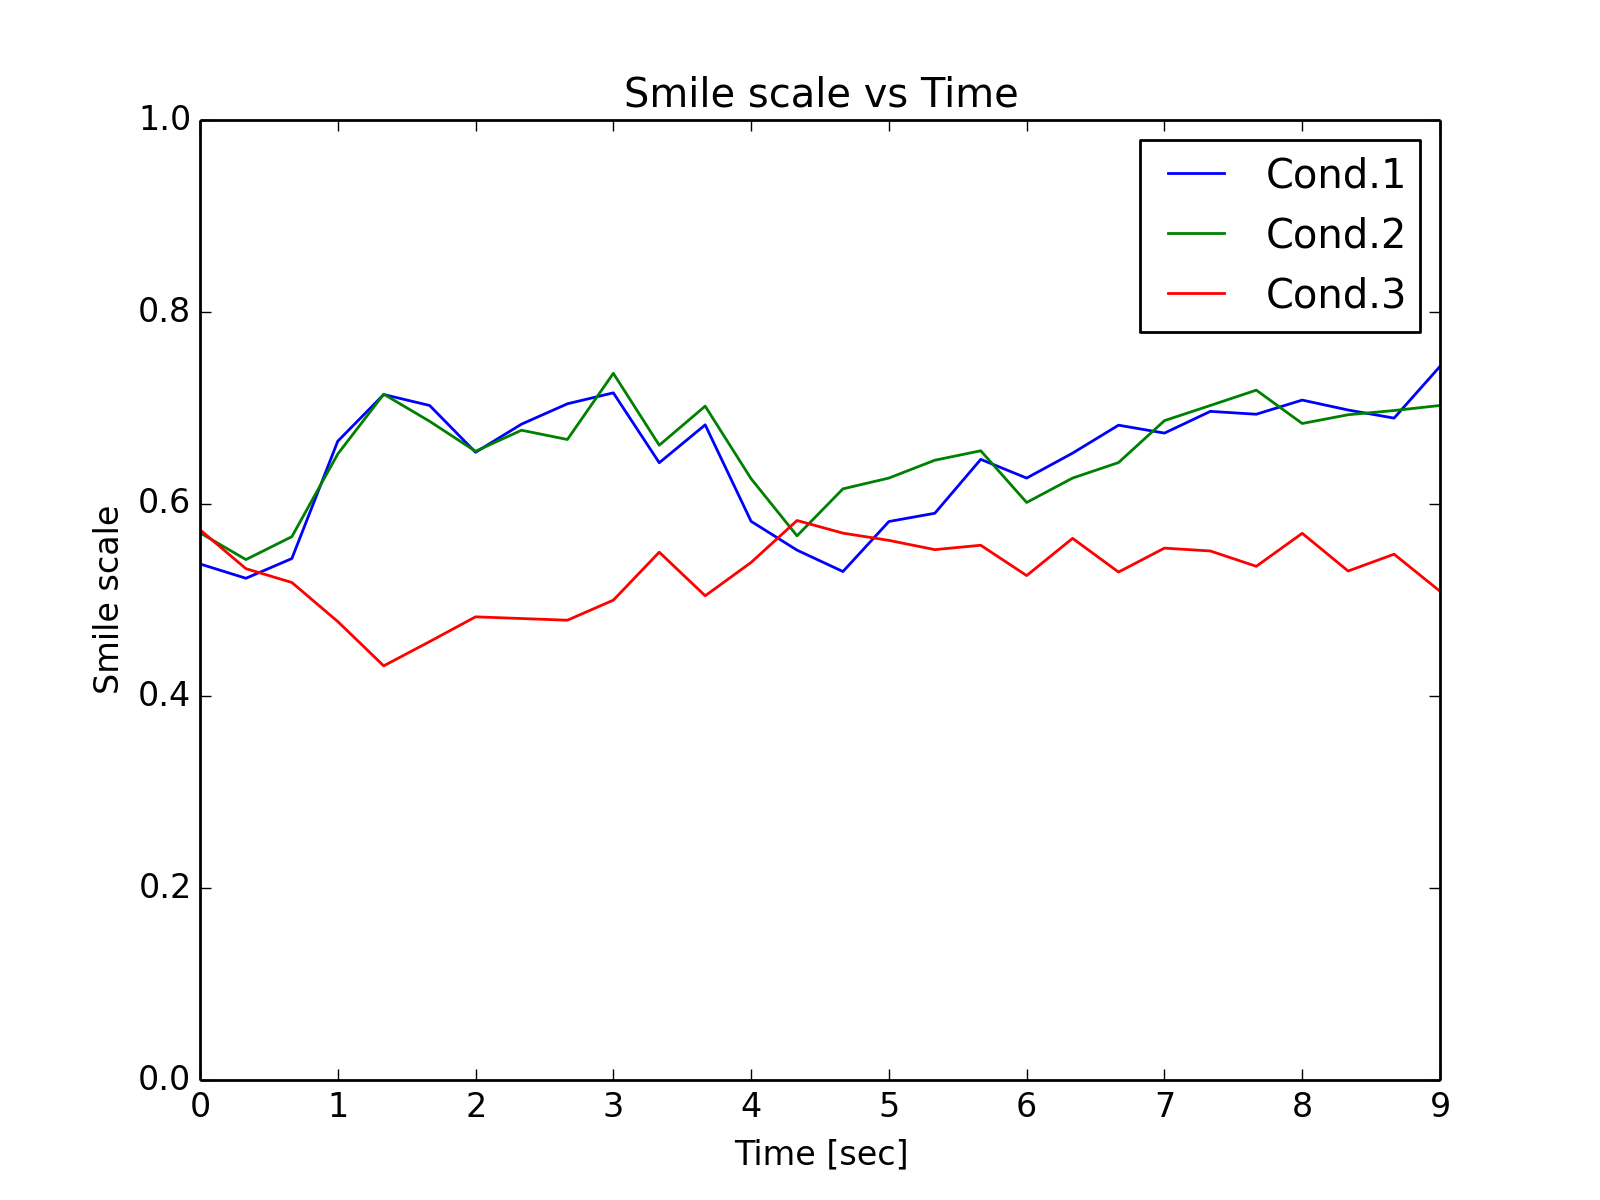
\includegraphics[width=140mm, bb=0 0 600 450]{images/smooth5_avg.png}
\caption{笑顔尺度の値の変化}
  \label{graph-smooth}
\end{figure}

\ref{手続き}節で述べたように,音声が流れる前には被験者は作り笑いを作っている.図\ref{graph-smooth}からは,音声が流れ始めてすぐの 0.0-0.6秒 は条件間に差がほとんどなく,1.0-2.0秒ごろの条件間の差が最も大きいことが認められた.0.0-0.6秒の笑顔尺度の平均値を基準値として,1.0-2.0秒の笑顔尺度の値の平均値から基準値を減算した値は,音声による笑顔誘発の効果を表すと考えられる.この差の値についてShapiro-Wilkの方法を用いて正規性を検定したところ,正規性は認められなかった(p $<$ .05).この誘発効果を表す差が無いという帰無仮説をWilcoxonの符号付き順位和検定で検定したところ,条件1,2ではそれぞれ棄却された ($p<.05$) が,条件3では採択された.誘発効果を表す値の分布を図\ref{graph-diff}に箱ひげ図で描いた.

\begin{figure}[h!]
  \centering
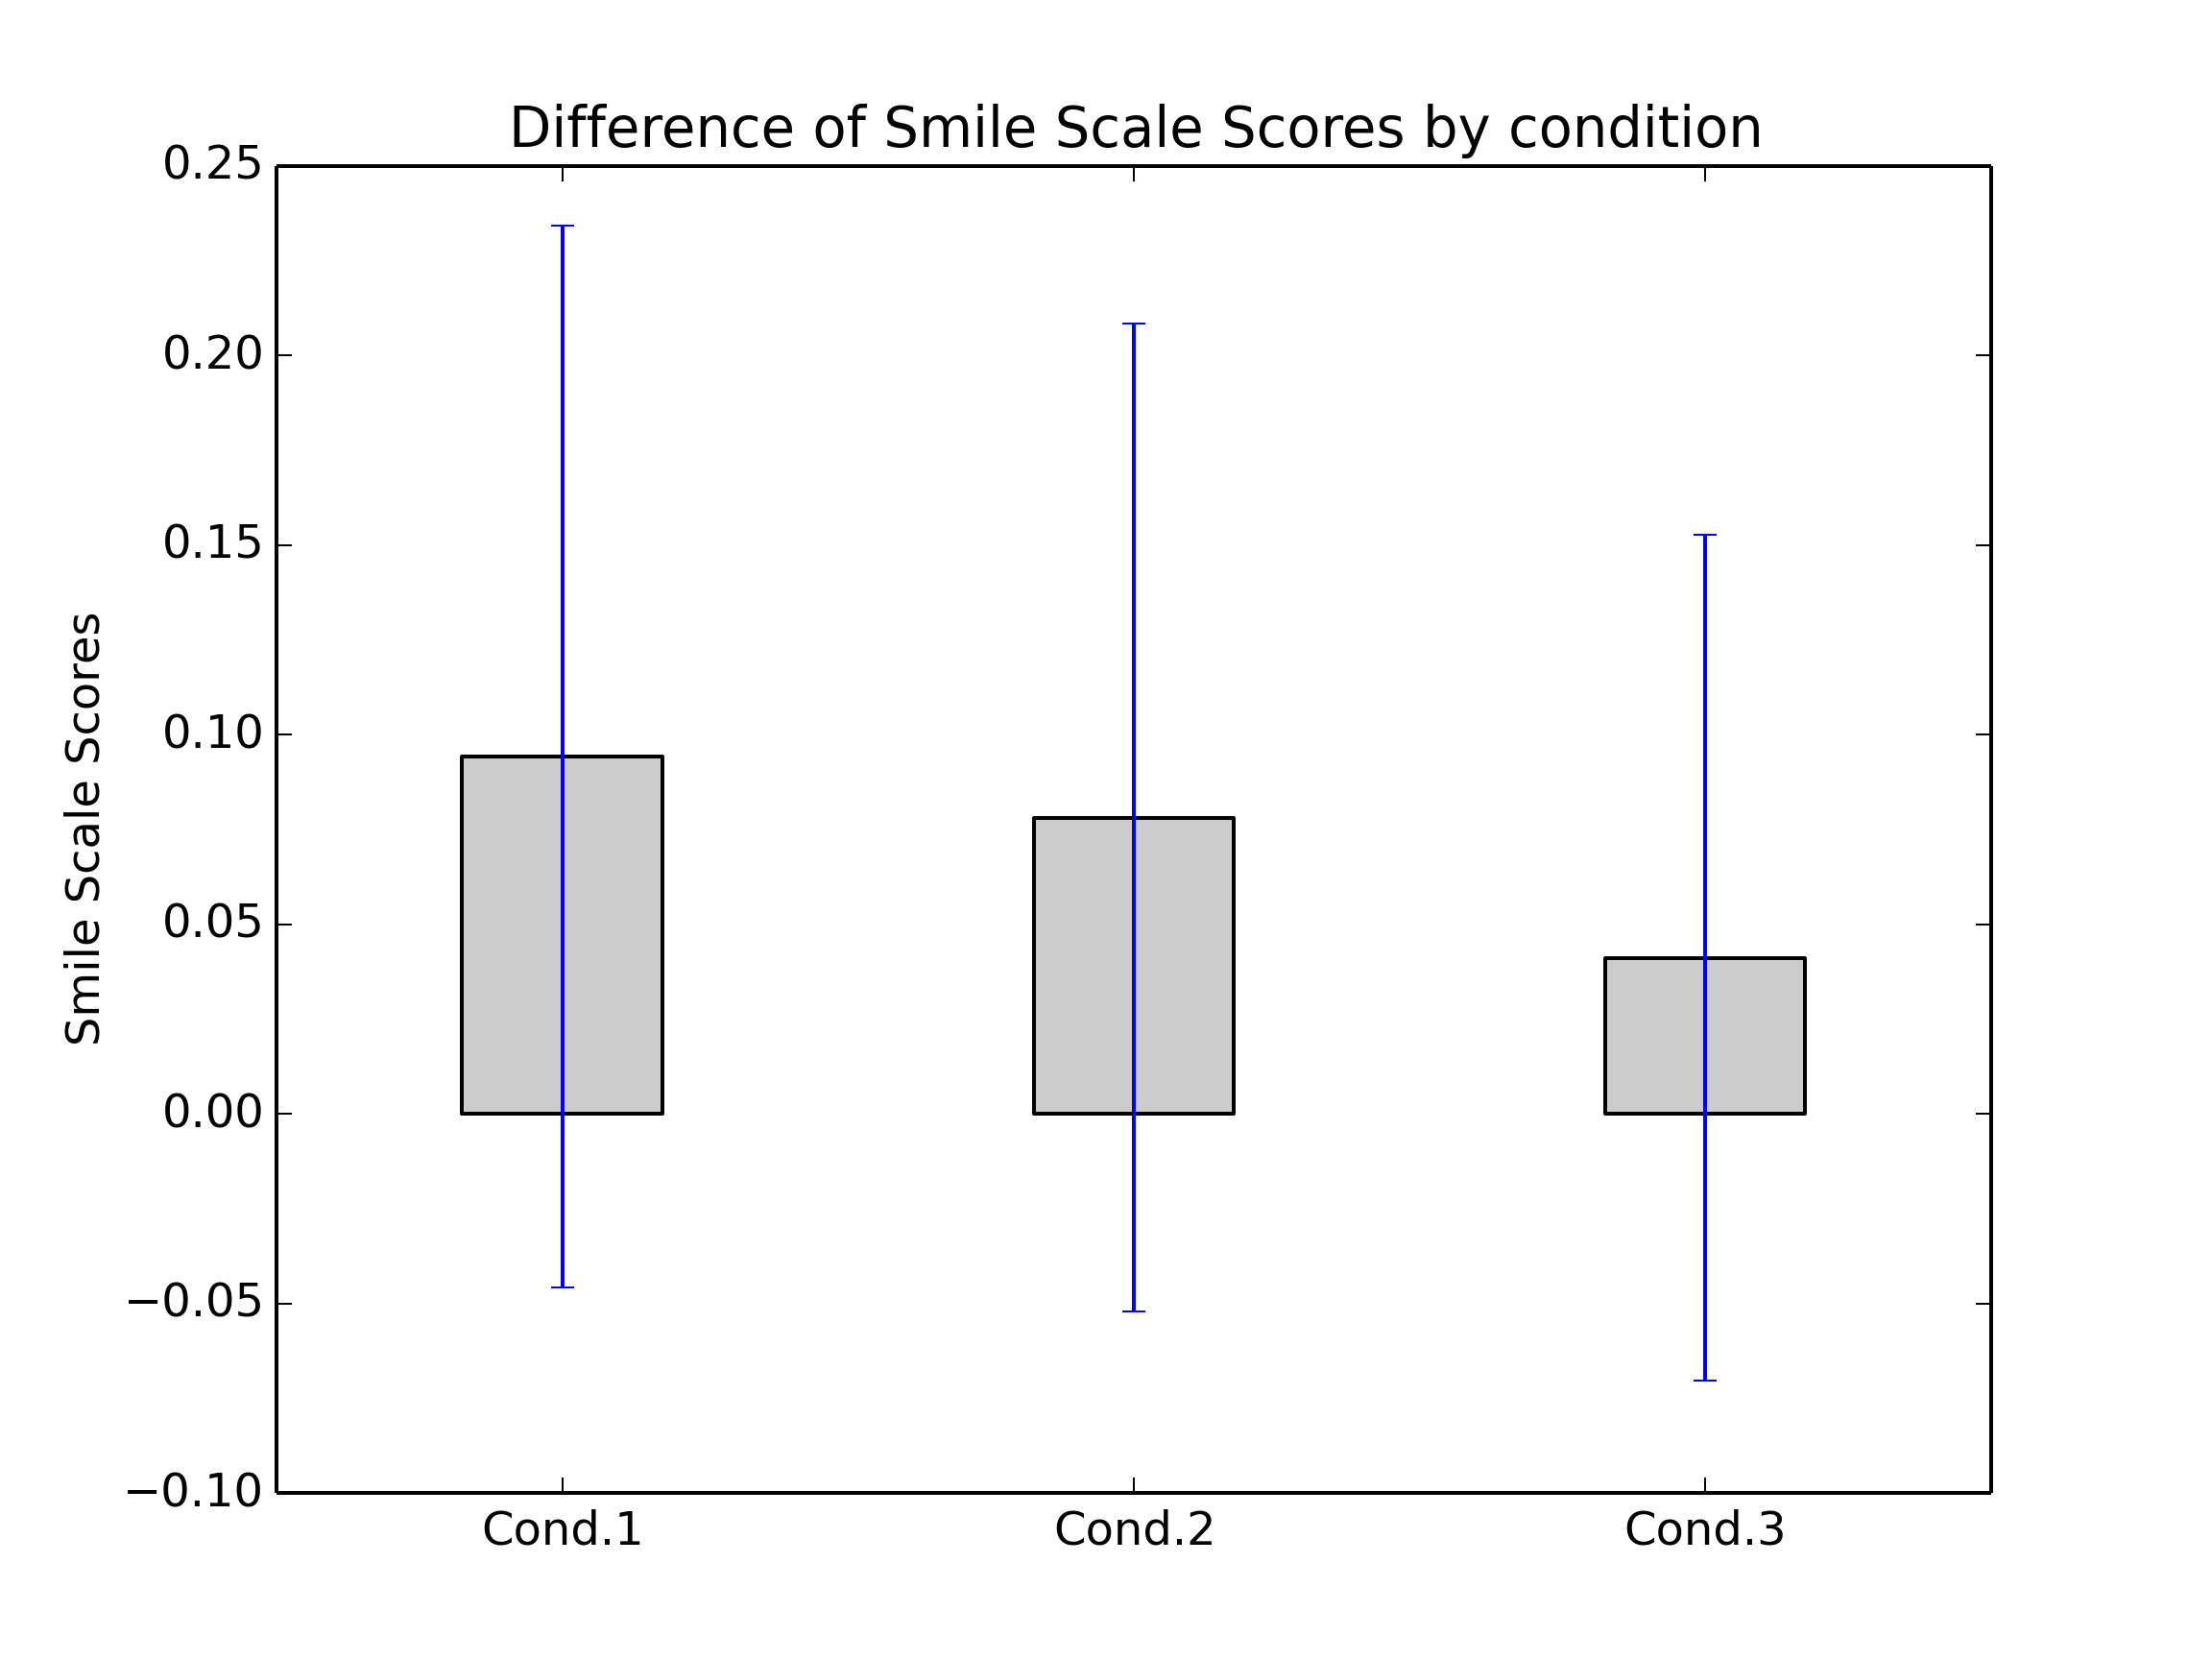
\includegraphics[width=140mm, bb=0 0 600 450]{images/graph-diff.png}
\caption{0.0-0.6sと1.0-2.0sの笑顔尺度の差の平均値}
  \label{graph-diff}
\end{figure}


さらに各条件で誘発効果に差があるか調べるため,誘発効果を表す値について各条件群についてKruskal-WallisのH検定を行った結果,群間の平均値に有意に差があるという結果が出た ($p<.05$).2条件間でWilcoxonの符号付き順位和検定を行ったところ,条件1-条件3, 条件2-条件3の間に有意に差があった ($p<.05$, 表\ref{anova-p}).

\break
\begin{table}[htb]
  \begin{center}
    \caption{Wilcoxonの符号付き順位和検定の結果}
    \begin{tabular}{|c|c|r||r|} \hline
      群 & $p$値  \\ \hline  \hline
      条件1(青年笑い声)-条件2(幼児笑い声) & $0.86$ \\ \hline
      条件2(幼児笑い声)-条件3(シャッター音) & $0.03$ \\ \hline
      条件1(青年笑い声)-条件3(シャッター音) & $0.04$ \\ \hline
    \end{tabular}
    \label{anova-p}
  \end{center}
\end{table}


また,笑い誘発の男女差を確認するため,各条件の誘発効果を表す値についての男女差を,Mann-WhitneyのU検定を用いて検定した結果を表\ref{manw}に示す.条件1 (青年笑い声) については女性のほうが,条件3 (シャッター音) については男性のほうが,それぞれ有意に笑顔が誘発されやすい (いずれも$p<.05$, 片側検定)という結果となった.

\begin{table}[htb]
  \begin{center}
    \caption{Mann-WhitneyのU検定の結果}
    \begin{tabular}{|c|c|c|}  \hline
      群 & p値 & 片側検定の方向 \\ \hline \hline
      条件1 (青年笑い声) & $0.037$ & (男性) $<$ (女性) \\ \hline
      条件2 (幼児笑い声)  & $0.156$ & (男性) $<$ (女性) \\ \hline
      条件3 (シャッター音) & $0.046$ & (男性) $>$ (女性) \\ \hline
    \end{tabular}
    \label{manw}
  \end{center}
\end{table}


さらに,音声の種類の違いが笑顔誘発の度合いに及ぼす影響の男女差を調べるため,誘発効果を表す値の2条件間の被験者内の差について,男女差があるかを,Mann-WhitneyのU検定を用いて確認した.条件1(青年笑い声) の誘発笑いの笑顔尺度と,条件2(幼児笑い声)の誘発笑いの笑顔尺度の符号を考慮した差は,女性のほうが有意に大きい ($p<.05$)が,ほかの2条件間では男女差は見られなかった.この結果は女性は比較的青年よりも幼児の笑い声に笑いを誘発され,男性はその逆の傾向があることを示唆する.

%結果を\ref{pair-genderdiff}に示す.

%\begin{table}[htb]
%  \begin{center}
%    \caption{マン・ホイットニーのU検定の結果 (p値)}
%    \begin{tabular}{|l|c|r||r|} \hline
%      (条件1) - (条件2) & $0.024$ & (男性) $>$ (女性) \\ \hline
%      (条件2) - (条件3) & $0.266$ & (男性) $<$ (女性) \\ \hline
%      (条件3) - (条件1) & $0.056$ & (男性) $>$ (女性) \\ \hline
%    \end{tabular}
%    \label{pair-genderdiff}
%  \end{center}
%\end{table}

最後に,代表的な画像を図\ref{nagatatsu2}, \ref{nagatatsu3}に示す.いずれも音声が流れ始めてから1.5秒後の写真である.

\begin{figure}[h!]
\begin{minipage}{0.49\columnwidth}
\begin{center}
\includegraphics[width=45mm, bb=0 0 768 1024]{images/nt2.jpg}
\end{center}
\caption{条件2 (笑顔尺度$:$0.97)}
\label{nagatatsu2}
\end{minipage}
\begin{minipage}{0.49\columnwidth}
\begin{center}
\includegraphics[width=45mm, bb=0 0 768 1024]{images/nt3.jpg}
\end{center}
\caption{条件3 (笑顔尺度$:$0.60)}
\label{nagatatsu3}
\end{minipage}
\end{figure}


\subsection{内観報告}

女性2名から,男性の笑い声は不快だという意見があった.また女性2名から,男性青年の笑い声よりも赤ちゃんのほうが笑いやすいという意見があった.そのうち1名は,それは自分が女性だからではないかという意見を付した.これらの報告は,実際に女性では青年より幼児の方が笑顔尺度の誘発度合いが大きかったことと符合する.

また男性のうち2名は,「いつも写真に撮られるくらいの笑顔で映ってください」という教示に対し,「いつも写真には笑顔では映らない」と応えたため,「それでは,いつも写真に取られる表情で写ってください」と指示した.今回の実験では,このような被験者に対する対応は準備していなかった.彼らの画像はRekognition APIで分析してもほとんど時間・条件間で違いが見られなかった.

男性のうち多くは,動画の撮影中に笑いを我慢し,撮影が終了したあと吹き出すように・こらえていた笑いを解放するように笑った.実験室という環境の緊張や,羞恥心などの抑制的な感情から,動画の撮影中に笑うことを我慢していたと報告した男性がいた.これに比べて女性は動画の終了を待たず笑顔になった場合が多かった.

\subsection{まとめ}

本システムにおいて,条件1(青年笑い声),条件2(幼児笑い声)で笑顔を誘発できていること,さらに対照とした条件3ではその効果が現れないことを検証した.また,男性青年の笑い声よりも幼児の笑い声のほうが笑顔を誘発しやすい傾向が女性では強かった.

また,笑顔の誘発にはディレイが存在し,誘発された笑顔が最も顕著になるのは条件1, 条件2ともに音声再生からおよそ1.0秒から2.0秒後であることがわかった.実際の写真撮影システムを構築する場合は,この結果を元にシャッターを切る時間を設定すれば良い.ただし,この値は再生する音声によって大きく異なるだろうから,異なる音声を扱う場合には今回のような実験を繰り返す必要がある.

比較可能な尺度としてRekognition APIの笑顔尺度を利用した.Rekognition を公開しているOrbeus社は,機械学習を用いた顔認識エンジン専業の企業で,多数の企業に顔認識システムを提供している\cite{Orbeus}.ただし笑顔尺度分析の科学的基礎づけは公開されておらず,この値の信頼性に対して評価を加えることは難しい.しかし連続した表情の変化に対して,ほぼ連続した値が得られていることから,ある程度信頼できるものと考えられる.



\section{結論}

本研究ではでは、シャッターを切る前に笑い声を再生することで自然な笑顔を撮影するカメラシステムを提案し,スマートフォン上で動作するアプリケーションとして実装した.このシステムの有効性を検証するべく,コンピュータビジョンを用いた笑顔尺度測定で,実際に笑顔が撮影できたことを確認した.

\section{今後の研究計画}

今後は以下について検討する.

\begin{itemize}
\item 今回コンピュータビジョンを用いて評価した笑顔画像の自然さを,人間の被験者に評価させる実験を計画している.まず撮影された画像群をシークさせながら最も自然な笑顔が撮影された音声再生からの時間遅れを特定し,さらに各条件について自然さを2択強制選択によって評価させる.
\item 今回利用したモーダルは聴覚のみだったが,笑い誘発効果は笑い行動の動画でも引き起こせるはずである.インカメラを用いて,笑っている人の動画を見せて笑顔を誘発するカメラは容易に実現でき,応用可能性も広がる.音声のみの場合と効果を比較したい.
\item Kleinke らは,自身の笑顔を鏡を通して見ることでポジティブな気分が増幅されることを実験で示した\cite{kleinke1998effects}.Yoshidaらは,変形させた自分の表情をフィードバックすることで,情動体験をポジティブ/ネガティブに操作できることを示した\cite{Yoshida2013}.誘発された笑顔を被撮影者にリアルタイムに呈示することで,ポジティブな情動体験を誘発することが可能だろう.
\item 本システムでは,被撮影者から見て笑い声の主体がはっきりしなかった.ぬいぐるみに本システムを埋め込んで,ぬいぐるみのキャラクターの笑い声の音声を流すなどして,主体をはっきりと認知させるとより笑顔を誘発できるのかを調査したい.
\item 本システムはテーマパークや観光地での顔ハメなど,もともと記念撮影行為が多く見られるシチュエーションでの利用に適している.そのような場面で着ぐるみやアトラクション,顔ハメ本体にシステムを埋め込むことで,良い笑顔が撮れる記念撮影スポットができるだろう.
\item 本システムで写真を撮影したあと,笑いを誘発された条件下では「ニヤニヤしてしまい,あまり良い笑顔にならなかった」という報告をした被験者がいた.この被験者に撮影できた画像を見せたところ,予想していたよりも好ましい笑顔が撮影できていたという感想が得られた.ユーザスタディとして,被験者に「どの条件がいちばん自然な笑顔が撮れていると思うか」を予想させたあと,条件との対応を隠したまま実際の写真を見せ,どれがいちばん自然な表情を評価させることで,自身の表情の主観的な評価と,実際に撮影された写真に対する評価のズレを検討したい.
\end{itemize}


\section{発表文献}

\begingroup
\renewcommand{\section}[2]{}%
\begin{thebibliography}{9}
  \bibitem{Fushimi2014} 伏見 遼平, 福嶋 政期, 苗村 健, "笑い声呈示により自然な笑顔を撮影するカメラの提案'', \textsl{EC2014: エンタテインメントコンピューティング2014}. pp.26--31, 2014年9月.
\textgt{[EC2014デモ発表賞 受賞(2014.9.14)]}
\end{thebibliography}
\endgroup

\break
\bibliographystyle{unsrt}
\bibliography{InterimReport}

\end{document}
